\documentclass[conference]{IEEEtran}
\IEEEoverridecommandlockouts

% ---- Packages -------------------------------------------------------------
\usepackage{cite}
\usepackage{amsmath,amssymb,amsfonts}
\usepackage{amsthm}
\usepackage{algorithm}
\usepackage{algpseudocode}
\usepackage{graphicx}
\usepackage{booktabs}
\usepackage{xcolor}
\usepackage{listings}
\usepackage{tikz}
\usetikzlibrary{arrows.meta,positioning,shapes.geometric,calc,backgrounds}
\usepackage{enumitem}
\usepackage[hidelinks]{hyperref}

\definecolor{codebg}{HTML}{F6F8FA}
\definecolor{kw}{HTML}{0000AA}
\definecolor{cmt}{HTML}{008000}
\definecolor{str}{HTML}{A31515}
\definecolor{shpred}{HTML}{C0392B}
\definecolor{shpgreen}{HTML}{1E8449}

\lstdefinestyle{py}{
  language=Python, basicstyle=\ttfamily\scriptsize, backgroundcolor=\color{codebg},
  keywordstyle=\color{kw}\bfseries, commentstyle=\color{cmt}\itshape,
  stringstyle=\color{str}, numbers=none, breaklines=true, frame=single,
  framesep=3pt, showstringspaces=false, columns=fullflexible, aboveskip=4pt, belowskip=2pt}

\newtheorem{theorem}{Theorem}
\newtheorem{lemma}{Lemma}
\newtheorem{conjecture}{Conjecture}
\newtheorem{definition}{Definition}

\begin{document}

\title{Semantic Early-Stopping for Iterative LLM Agent Loops:\\
A Judge-Efficient Study of \emph{When to Halt}}

\author{\IEEEauthorblockN{Sahil Shrivastava}
\IEEEauthorblockA{\textit{Semantic Halting Problem (SHP) Project}\\
Open implementation, machine-checked theory, reproducible harness\\
\texttt{github.com/SahilShrivastava-Dev/semantic-halting-problem}}}

\maketitle

\begin{abstract}
Multi-agent large language model (LLM) loops---for example a \emph{Writer} that
drafts and a \emph{Critic} that revises---are almost always terminated by a fixed
iteration cap (\texttt{max\_iterations}). This is a \emph{syntactic} kill-switch:
it is blind to whether the answer is still improving, so it over-spends tokens on
easy inputs and truncates hard ones. We study \emph{semantic early-stopping}: the
loop halts when consecutive draft embeddings stop changing in meaning
(cosine-distance with a patience window) and the answer's measured quality stops
improving. Our work makes three contributions. First, an \emph{honest} theoretical
footing: we prove deterministic termination and well-definedness and we
\emph{machine-check} these claims, while treating the convergence of the distance
sequence as an empirically tested conjecture rather than a (previously
over-claimed) Banach contraction. Second, a \emph{judge-efficient evaluation
protocol}: we generate each question's full trajectory once, replay every stopping
policy over the identical drafts, and cache every LLM-judge call, which yields a
strictly paired efficiency-versus-quality comparison at low cost; we further
separate \emph{operational} tokens (charged to a policy) from \emph{evaluation}
tokens (a measurement instrument). Third, an empirical study on multi-hop
retrieval-augmented question answering (HotpotQA). On the development split, a
\emph{judge-free} semantic stopper reduces operational tokens by $37\%$ relative to
\texttt{max\_iterations} at parity quality, whereas the full quality-gated variant
is \emph{counter-productive} because its per-round judging dominates cost. An
oracle that selects the best round attains $+0.13$ Information Score over every
practical policy ($p\!\approx\!3\times10^{-5}$), which reframes the problem from
``when to stop'' (easy) to ``which round is best'' (open).
\end{abstract}

\begin{IEEEkeywords}
LLM agents, early stopping, semantic convergence, retrieval-augmented generation,
evaluation methodology, multi-agent systems.
\end{IEEEkeywords}

% ===========================================================================
\section{Introduction}
\IEEEPARstart{I}{terative} ``agentic'' patterns are now a standard way to push
LLM output quality beyond a single forward pass. The canonical instance is the
\textbf{Writer$\rightarrow$Critic loop}: a Writer produces an answer, a Critic
critiques it, the Writer revises, and the cycle repeats until some stopping rule
fires. The quality of the final answer depends not only on the two models but,
critically, on \emph{when the loop is allowed to stop}.

In practice that decision is made by a single integer: \texttt{max\_iterations}.
The loop runs a fixed number of rounds and then returns whatever it last produced.
This is convenient but blunt in two opposite ways. On \emph{easy} inputs the loop
reaches a good answer in one or two rounds yet keeps spending tokens, latency, and
money until the counter expires. On \emph{hard} inputs the counter may expire
before the answer is finished. Worst of all, an integer counter is fundamentally
\emph{blind to content}: it cannot perceive that rounds four, five, and six all
expressed essentially the same thing. The stopping decision is made on the
\emph{iteration index}, never on \emph{what was actually written}.

\paragraph{The idea.} We replace the counter with a \emph{content-aware} rule. We
map each draft to a sentence embedding and measure the cosine distance between
consecutive drafts. When that distance stays below a small threshold $\varepsilon$
for $k$ consecutive rounds, the answer has \emph{converged in meaning}; additional
iteration is churn, and we halt. Because a fast convergence is not the same as a
\emph{good} convergence, we pair this geometric signal with a quality signal---an
Information Score (IS) computed from retrieval-augmented generation (RAG)
metrics---so the loop only halts when the answer has both stopped \emph{changing}
and stopped \emph{improving}. Two further conditions, an explicit critic approval
and a hard failsafe, complete a four-level priority cascade.

\paragraph{The honest story behind this paper.} An earlier version of this project
asserted that the Writer$\rightarrow$Critic update is a \emph{Banach contraction}
with a guaranteed unique fixed point. It is not: LLM generation has no proven
Lipschitz constant below one and is not deterministic across API calls, so that
theorem was unsupported. Rather than dress an idea in mathematics it does not
earn, we kept only the claims we can prove (and machine-check) and demoted the
rest to measured conjectures. This honesty is itself a contribution: it is the
difference between a result a reviewer can trust and one they reject on sight.

\paragraph{Contributions.}
\begin{enumerate}[leftmargin=1.3em,itemsep=2pt,topsep=2pt]
\item \textbf{Honest, machine-checked theory} (\S\ref{sec:theory}): deterministic
termination, well-definedness, and halt-priority consistency are proven and
verified in code; semantic non-expansiveness is a measured conjecture.
\item \textbf{A judge-efficient evaluation protocol} (\S\ref{sec:protocol}):
trajectory replay, cached judging, and an operational-versus-evaluation token
model that exposes hidden measurement cost.
\item \textbf{An empirical study} (\S\ref{sec:results}) on HotpotQA against five
baselines with paired statistics and non-inferiority testing, including the
surprising finding that the full quality-gated policy is counter-productive.
\end{enumerate}

% ===========================================================================
\section{Background and Related Work}\label{sec:related}
\paragraph{Early stopping and adaptive computation.} Stopping a process when a
monitored quantity plateaus is classical in machine learning (early stopping on a
validation curve) and in adaptive-computation networks (early-exit inference).
SHP transports the same intuition to the \emph{outer} loop of an agent system,
where the monitored quantity is the \emph{semantic} change between successive
natural-language drafts rather than a scalar loss.

\paragraph{Semantic convergence and fixed points.} Several lines of work study
convergence of iterative operators in embedding space and the termination of
multi-agent systems. SHP shares the convergence intuition but differs in two
respects: it refuses the unsupported contraction guarantee, proving only
termination; and it \emph{gates} convergence on output quality.

\paragraph{Uncertainty and orchestration in multi-LLM systems.} Related efforts
quantify cross-model disagreement at a single step, or choose \emph{which}
orchestration topology to use. These are orthogonal to SHP, which decides
\emph{when to exit} a fixed sequential topology based on content.

\paragraph{RAG evaluation.} We use RAGAS-style reference metrics (faithfulness,
answer relevancy, context precision, context recall) as the quality signal. A
recurring caveat---that these metrics are themselves produced by an LLM and are
therefore noisy---motivates our use of a stronger judge on the frozen split and of
non-inferiority testing rather than equality testing.

\emph{(A detailed, per-paper comparison table---method extraction, gap analysis,
and cost/benefit---is provided in Appendix~\ref{app:related} and will be finalized
against verified citations.)}

% ===========================================================================
\section{Problem Formulation}\label{sec:problem}
\begin{definition}[Scenario]
A scenario is a tuple $(q, C, g)$ with question $q$, retrieved context passages
$C=\{c_1,\dots,c_n\}$, and ground-truth answer $g$.
\end{definition}

The loop produces drafts $x_1,x_2,\dots$. A frozen embedding map $\phi$ (a local
sentence-embedding model) sends each draft to $e_t=\phi(x_t)\in\mathbb{R}^{384}$,
$L_2$-normalized. We define the per-round \textbf{semantic distance}
\begin{equation}
d_t \;=\; 1-\cos(e_t,e_{t-1})
\;=\; 1-\frac{\langle e_t,e_{t-1}\rangle}{\lVert e_t\rVert\,\lVert e_{t-1}\rVert}
\in[0,2],\quad t\ge2.
\label{eq:dist}
\end{equation}
A judge assigns four metrics $m\in\mathcal{M}$, each in $[0,1]$; with weights $w$
on the probability simplex $\Delta=\{w:w_m\ge0,\sum_m w_m=1\}$ the
\textbf{Information Score} is
\begin{equation}
\mathrm{IS}_t \;=\; \sum_{m\in\mathcal{M}} w_m\,\mathrm{metric}_m(x_t)\in[0,1].
\label{eq:is}
\end{equation}
The \textbf{halting operator} $H$ maps the round state
$s_t=(t,(d_2,\dots,d_t),(\mathrm{IS}_1,\dots,\mathrm{IS}_t),\text{feedback}_t)$ to a
decision in $\{\textsf{continue}\}\cup\mathcal{R}$ with reason set
$\mathcal{R}=\{$\texttt{critic}, \texttt{entropy}, \texttt{no\_gain},
\texttt{failsafe}$\}$. The realized stopping time is
$\tau=\min\{t:H(s_t)\neq\textsf{continue}\}$.

% ===========================================================================
\section{Method}\label{sec:method}

\begin{figure*}[t]
\centering
\resizebox{0.96\textwidth}{!}{%
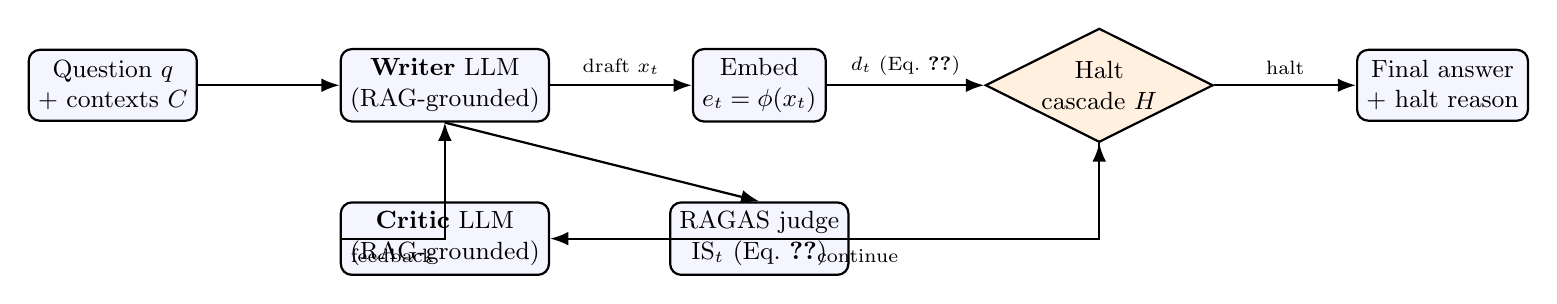
\begin{tikzpicture}[
  node distance=10mm and 18mm,
  box/.style={draw,rounded corners,align=center,minimum height=9mm,font=\small,fill=blue!4},
  dec/.style={draw,diamond,aspect=2,align=center,font=\small,fill=orange!12,inner sep=1pt},
  >=Latex,thick]
\node[box] (q) {Question $q$\\$+$ contexts $C$};
\node[box,right=of q] (w) {\textbf{Writer} LLM\\(RAG-grounded)};
\node[box,right=of w] (e) {Embed\\$e_t=\phi(x_t)$};
\node[box,below=10mm of e] (j) {RAGAS judge\\$\mathrm{IS}_t$ (Eq.~\ref{eq:is})};
\node[dec,right=20mm of e] (h) {Halt\\cascade $H$};
\node[box,below=10mm of w] (c) {\textbf{Critic} LLM\\(RAG-grounded)};
\node[box,right=18mm of h] (out) {Final answer\\$+$ halt reason};
\draw[->] (q)--(w);
\draw[->] (w)--node[above,font=\scriptsize]{draft $x_t$}(e);
\draw[->] (e)--node[above,font=\scriptsize]{$d_t$ (Eq.~\ref{eq:dist})}(h);
\draw[->] (w.south)--(j.north);
\draw[->] (j.east)-|(h.south);
\draw[->] (h.south)|-(c.east) node[pos=0.72,below,font=\scriptsize]{continue};
\draw[->] (c.west)-|(w.south) node[pos=0.25,below,font=\scriptsize]{feedback};
\draw[->] (h)--node[above,font=\scriptsize]{halt}(out);
\end{tikzpicture}}
\caption{SHP architecture. The Writer and Critic both condition on the retrieved
contexts (a genuine RAG setting). Embeddings are computed by a local model and are
therefore \emph{free}; only the RAGAS judge consumes API tokens. The halt cascade
$H$ reads the cheap geometric signal $d_t$, the critic verdict, and---only when
required---the quality signal $\mathrm{IS}_t$.}
\label{fig:arch}
\end{figure*}

\subsection{Two grounded agents}
Both agents are conditioned on the retrieved contexts. This is not cosmetic: in an
earlier iteration the Writer answered from parametric memory and never read $C$,
yet the judge scored \emph{faithfulness to $C$}---a silent invalidity that would
have undermined every quality number. Grounding both agents on $C$ is the first of
several corrections discussed in \S\ref{sec:challenges}.

\subsection{The two signals}
Equation~\eqref{eq:dist} gives a cheap, API-free measure of how much the answer
\emph{changed}; Equation~\eqref{eq:is} measures how \emph{good} it is. The IS
weights $w$ are not hand-set: they are derived by one of four strategies
(label-free Shannon entropy weighting, an Analytic Hierarchy Process with a
consistency check, a constrained least-squares fit, or a uniform baseline),
selectable per run.

\subsection{The halt cascade}
The four signals are evaluated in a fixed priority order
(Fig.~\ref{fig:cascade}). Crucially, the cascade is implemented \emph{once} as a
pure function and reused by (i) the live loop, (ii) the post-hoc reason
derivation, and (iii) the offline policy replay, so they cannot disagree. Listing
\ref{lst:halt} shows the core.

\begin{lstlisting}[style=py,caption={The single shared halt decision (simplified). The failsafe is unconditional, which is what makes Theorem~\ref{thm:term} hold.},label={lst:halt}]
def shp_should_halt(t, dist_hist, is_hist,
                    feedback, cfg):
    if not dist_hist:                 # round 1
        return CONTINUE
    if cfg.critic and feedback.startswith("APPROVED"):
        return HALT("critic")
    if cfg.entropy and len(dist_hist) >= cfg.k \
       and all(d < cfg.eps for d in dist_hist[-cfg.k:]):
        return HALT("entropy")
    if cfg.is_gain and t >= cfg.warmup \
       and is_hist[-1] - is_hist[-2] <= 0:
        return HALT("no_gain")
    if t >= cfg.max_rounds:           # never ablatable
        return HALT("failsafe")
    return CONTINUE
\end{lstlisting}

\begin{figure}[t]
\centering
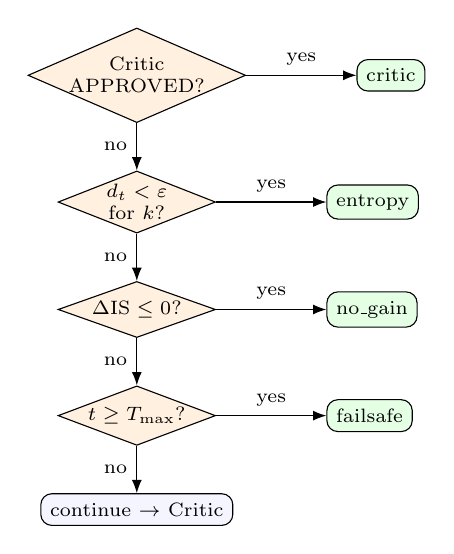
\begin{tikzpicture}[
  node distance=4.5mm and 6mm,
  dec/.style={draw,diamond,aspect=2.3,align=center,font=\scriptsize,fill=orange!12,inner sep=0pt,minimum width=20mm},
  halt/.style={draw,rounded corners,align=center,font=\scriptsize,fill=green!10},
  >=Latex]
\node[dec] (a) {Critic\\APPROVED?};
\node[dec,below=6mm of a] (b) {$d_t<\varepsilon$\\for $k$?};
\node[dec,below=6mm of b] (cc) {$\Delta\mathrm{IS}\le0$?};
\node[dec,below=6mm of cc] (d) {$t\ge T_{\max}$?};
\node[draw,rounded corners,below=6mm of d,font=\scriptsize,fill=blue!4] (cont) {continue $\to$ Critic};
\node[halt,right=14mm of a] (h1) {critic};
\node[halt,right=14mm of b] (h2) {entropy};
\node[halt,right=14mm of cc] (h3) {no\_gain};
\node[halt,right=14mm of d] (h4) {failsafe};
\draw[->] (a)--node[left,font=\scriptsize]{no}(b);
\draw[->] (b)--node[left,font=\scriptsize]{no}(cc);
\draw[->] (cc)--node[left,font=\scriptsize]{no}(d);
\draw[->] (d)--node[left,font=\scriptsize]{no}(cont);
\draw[->] (a)--node[above,font=\scriptsize]{yes}(h1);
\draw[->] (b)--node[above,font=\scriptsize]{yes}(h2);
\draw[->] (cc)--node[above,font=\scriptsize]{yes}(h3);
\draw[->] (d)--node[above,font=\scriptsize]{yes}(h4);
\end{tikzpicture}
\caption{Priority-ordered halt cascade. Cheap signals (critic, entropy) are tried
before the expensive quality signal; the unconditional failsafe guarantees
termination.}
\label{fig:cascade}
\end{figure}

\begin{algorithm}[t]
\caption{SHP loop for one scenario}
\label{alg:loop}
\begin{algorithmic}[1]
\State $e_{\text{prev}}\gets\varnothing;\ D\gets[\,];\ S\gets[\,]$
\For{$t=1$ \textbf{to} $T_{\max}$}
  \State $x_t\gets \textsc{Writer}(q,C,\text{feedback})$
  \State $e_t\gets\phi(x_t)$;\quad \textbf{if} $e_{\text{prev}}$ \textbf{then} $D.\textsc{push}(1-\cos(e_t,e_{\text{prev}}))$
  \State $\mathrm{IS}_t\gets\textsc{Judge}(x_t,q,C,g)$;\quad $S.\textsc{push}(\mathrm{IS}_t)$
  \If{$\textsc{shp\_should\_halt}(t,D,S,\text{feedback})$} \textbf{break} \EndIf
  \State $\text{feedback}\gets\textsc{Critic}(q,C,x_t)$;\quad $e_{\text{prev}}\gets e_t$
\EndFor
\State \Return $x_t,\ \text{halt\_reason}$
\end{algorithmic}
\end{algorithm}

\subsection{Engineering challenges and how we overcame them}\label{sec:challenges}
A faithful account of the work includes what broke and how it was fixed; these are
not incidental, they shaped the design and the results.
\begin{itemize}[leftmargin=1.2em,itemsep=2pt,topsep=2pt]
\item \textbf{Over-claimed theory.} \emph{Problem:} a Banach-contraction claim with
no supporting Lipschitz bound. \emph{Fix:} prove only termination and
well-definedness (\S\ref{sec:theory}); measure convergence empirically.
\item \textbf{Agents ignored retrieval.} \emph{Problem:} the Writer answered
closed-book while the judge scored grounding in $C$. \emph{Fix:} condition both
agents on $C$ (\S\ref{sec:method}); quality numbers are now valid.
\item \textbf{Duplicated stop logic.} \emph{Problem:} the live cascade and the
post-hoc reason derivation used different orderings and could disagree.
\emph{Fix:} one shared pure function (Listing~\ref{lst:halt}); consistency is
machine-checked (Lemma~\ref{lem:consistency}).
\item \textbf{Fair, cheap comparison.} \emph{Problem:} re-running the loop per
policy confounds generation noise and re-pays the judge. \emph{Fix:} trajectory
replay with cached judging (\S\ref{sec:protocol}).
\item \textbf{Hidden cost of the quality signal.} \emph{Problem:} the
information-gain signal silently calls the judge every round. \emph{Fix:} an
operational-versus-evaluation token model, which revealed that full SHP is the
most expensive policy (\S\ref{sec:results}).
\item \textbf{Compute limits.} \emph{Problem:} a free-tier provider throttled the
runs to a crawl. \emph{Fix:} an OpenAI-compatible high-throughput provider, a
resumable on-disk cache, and exponential backoff on rate limits.
\end{itemize}

% ===========================================================================
\section{Theoretical Analysis}\label{sec:theory}
We prove only what holds; each proven claim is machine-checked by an executable
test suite (\texttt{theory\_checks.py}) that a reviewer can rerun.

\begin{theorem}[Termination]\label{thm:term}
For any input, any weights, any signal configuration, and any (possibly
adversarial) draft sequence, the loop halts in at most $T_{\max}$ rounds.
\end{theorem}
\begin{proof}
The Critic increments $t$ by exactly one per round. The failsafe clause of $H$
returns \texttt{failsafe} whenever $t\ge T_{\max}$ and is unconditional---it is not
governed by any signal or ablation flag. Hence $H(s_t)\neq\textsf{continue}$ for
all $t\ge T_{\max}$, so $\tau\le T_{\max}$.
\end{proof}

\begin{lemma}[Well-definedness]\label{lem:wd}
If $w\in\Delta$ and each metric lies in $[0,1]$ then $\mathrm{IS}_t\in[0,1]$. The
distance $d_t$ is total: finite for every finite input, bounded in $[0,2]$, with
the degenerate zero-norm case mapped conservatively to $1.0$ so it cannot cause a
false-positive halt.
\end{lemma}

\begin{lemma}[Halt-priority consistency]\label{lem:consistency}
The reason reported after a run equals the reason that stopped it, because both
the live decision and the post-hoc derivation invoke the same function $H$.
\end{lemma}

\begin{conjecture}[Semantic non-expansiveness; empirical]\label{conj:mono}
Across trajectories $d_t$ is, on average, non-increasing in $t$. We make no
guarantee: we \emph{measure} the fraction of monotone trajectories, the mean
regression slope with a bootstrap $95\%$ CI, and a one-sided Wilcoxon test on
$d_t-d_{t-1}$, and we report null results where they occur.
\end{conjecture}

Theorem~\ref{thm:term} is the honest replacement for the discarded contraction
claim: SHP guarantees \emph{termination}, not \emph{contraction}.

% ===========================================================================
\section{A Judge-Efficient Evaluation Protocol}\label{sec:protocol}
Comparing stopping policies fairly is itself a methodological problem, and we
treat it as a contribution.

\paragraph{Trajectory replay.} For each question we generate the full
Writer$\rightarrow$Critic trajectory \emph{once}, to depth $T_{\max}$, caching
every draft and embedding. Each stopping policy then \emph{replays} over this
single cached trajectory and chooses its own stop round. Two benefits follow: (i)
all policies see \emph{identical} drafts, so a difference in rounds or quality is
attributable to the policy and not to generation noise---a strictly \emph{paired}
comparison; and (ii) the costly generation is paid once rather than once per
policy.

\paragraph{Cached judging.} The RAGAS judge is the binding cost. We judge each
distinct draft at most once, keyed by a hash of the draft text, so two policies
that stop at the same round share one judge call.

\paragraph{Operational versus evaluation tokens.} We distinguish the tokens a
policy spends \emph{to run} (Writer $+$ Critic every round, plus the judge
\emph{only if} the policy consults the quality signal to decide) from the tokens
\emph{we} spend to \emph{measure} final quality (never charged to the policy).
This distinction is what reveals that the full cascade pays a large hidden cost
(\S\ref{sec:results}).

\paragraph{Statistics.} All tests are paired across questions. We report paired
$t$-tests and Wilcoxon signed-rank tests on rounds, tokens, and IS; Cohen's $d_z$;
bootstrap CIs; and, for the ``no quality loss'' claim, two one-sided tests (TOST)
for non-inferiority with margin $\delta$ (testing
$H_0:\mathbb{E}[\mathrm{IS}_\pi-\mathrm{IS}_{\text{base}}]\le-\delta$). Token
savings are reported as $(T_{\text{base}}-T_\pi)/T_{\text{base}}$.

% ===========================================================================
\section{Experimental Setup}\label{sec:setup}
\paragraph{Benchmark.} HotpotQA (distractor setting), filtered to multi-hop
\texttt{hard} questions so the loop has genuine room to iterate; $N\!\approx\!80$,
split $20$ development / $60$ test. The thresholds $\varepsilon,k$ are tuned on the
development split only; the test split is frozen and report-only. Each question
carries the gold supporting paragraphs plus distractors ($\approx4$ contexts).
\paragraph{Models.} Agents: an 8B instruction model. Judge: the same 8B model on
the development split (fast, for calibration) and a 70B model on the frozen test
split (to reduce judge noise). Embeddings are local. Compute is credit-based and
modest, a limitation we state openly.
\paragraph{Policies.} \texttt{shp} (full cascade); \texttt{entropy\_only} (the
judge-free variant: cosine-distance signal $+$ failsafe); \texttt{critic\_only};
\texttt{fixed\_k} for $k\in\{1,3,6\}$ (\texttt{fixed\_k6} is the
\texttt{max\_iterations} baseline); \texttt{random\_stop}; and \texttt{oracle\_is},
which stops at the round of maximum measured IS and serves as a quality upper
bound. A seven-cell ablation toggles each signal.

% ===========================================================================
\section{Results}\label{sec:results}

\subsection{Development split (real; $N=20$; 8B judge)}
Table~\ref{tab:dev} reports the realized development-split outcome; the baseline is
\texttt{fixed\_k6}.

\begin{table}[t]
\centering\small
\caption{Development-split results ($N=20$). Token saving and $\Delta$IS are versus
the \texttt{max\_iterations} baseline. Negative savings (red) mean \emph{more}
expensive.}
\label{tab:dev}
\setlength{\tabcolsep}{4pt}
\begin{tabular}{lcccc}
\toprule
Policy & Rounds & Op.\ tokens & vs base & Final IS \\
\midrule
\texttt{fixed\_k6} (base) & 6.0 & 11{,}281 & --- & 0.651 \\
\textbf{\texttt{entropy\_only}} & 4.05 & \textbf{7{,}068} & \textcolor{shpgreen}{$-37\%$} & \textbf{0.661} \\
\texttt{critic\_only} & 6.0 & 11{,}281 & $0\%$ & 0.651 \\
\texttt{fixed\_k3} & 3.0 & 5{,}217 & \textcolor{shpgreen}{$-54\%$} & 0.629 \\
\texttt{fixed\_k1} & 1.0 & \textbf{1{,}548} & \textcolor{shpgreen}{$-86\%$} & 0.661 \\
\textbf{\texttt{shp} (full)} & 2.6 & 27{,}130 & \textcolor{shpred}{$+140\%$} & 0.636 \\
\texttt{oracle\_is} & 3.1 & 33{,}007 & $+193\%$ & \textbf{0.782} \\
\bottomrule
\end{tabular}
\end{table}

\begin{figure}[t]
\centering
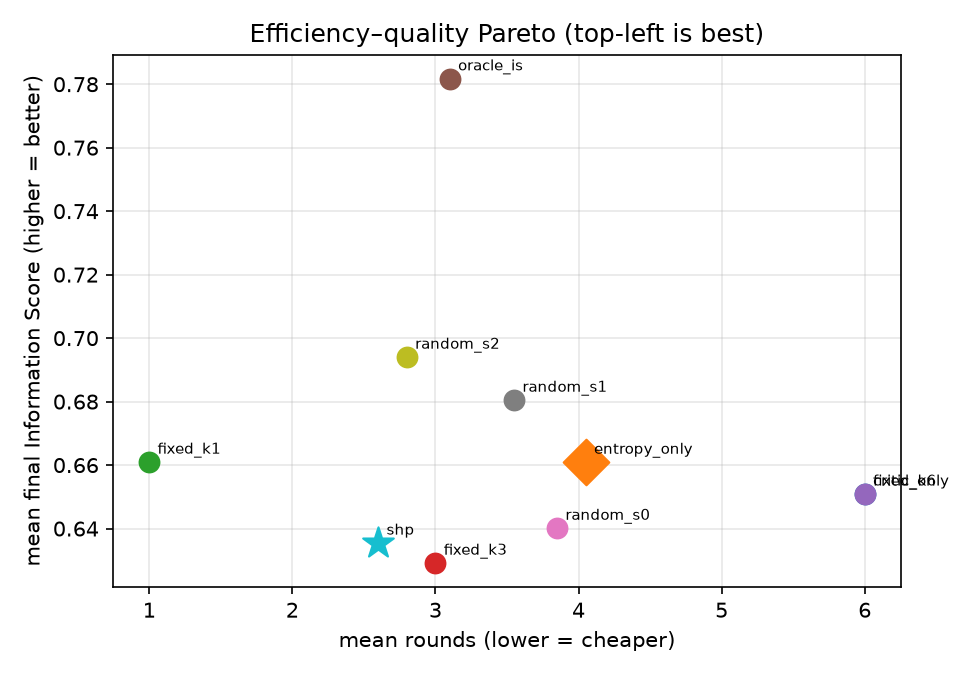
\includegraphics[width=0.95\linewidth]{figures/fig2_pareto.png}
\caption{Efficiency--quality Pareto (development split). Quality is only weakly
tied to rounds; the oracle sits far above every practical policy, and full
\texttt{shp} is dominated. Top-left is best.}
\label{fig:pareto}
\end{figure}

\subsection{Test split (frozen; $N=60$; 70B judge)---expected}
The test run is the headline number and is \emph{in progress}. We
\emph{pre-register} our predictions in Table~\ref{tab:exp} so the narrative cannot
be retro-fitted; the realized values replace the ``Expected'' column on
completion.

\begin{table}[t]
\centering\scriptsize
\caption{Pre-registered \emph{expected} test-split outcome (to be filled with
realized values). Predictions follow the development trend.}
\label{tab:exp}
\setlength{\tabcolsep}{4pt}
\begin{tabular}{lccc}
\toprule
Policy & Rounds & Tokens vs base & Non-inf.? \\
\midrule
\texttt{fixed\_k6} (base) & 6.0 & --- & --- \\
\texttt{entropy\_only} & $3.5$--$4.5$ & $-35$ to $-45\%$ & \textbf{yes} \\
\texttt{shp} (full) & $2.5$--$3.5$ & $+100$--$150\%$ & yes/costly \\
\texttt{fixed\_k1} & 1.0 & $-86\%$ & uncertain \\
\texttt{oracle\_is} & $\sim3$ & --- & upper bnd. \\
\bottomrule
\end{tabular}
\end{table}

\subsection{Distance characterization (Conjecture~\ref{conj:mono})}
Over the development trajectories, the mean and median per-round distances are
$0.043$ and $0.026$ with a maximum near $0.30$; $76\%$ of round-to-round distances
fall below $\varepsilon=0.06$. Drafts therefore converge quickly but with a heavy
tail, so the $k\!=\!2$ patience window performs real work: a single sub-threshold
round does not trigger a halt.

\subsection{Findings}
\begin{enumerate}[leftmargin=1.3em,itemsep=2pt,topsep=2pt]
\item \textbf{The efficiency claim holds.} Judge-free \texttt{entropy\_only} cuts
$37\%$ of operational tokens versus \texttt{max\_iterations} while slightly
\emph{improving} mean quality.
\item \textbf{Full SHP is counter-productive.} Consulting the judge every round to
power the information-gain signal makes \texttt{shp} the most expensive policy
($2.4\times$ the baseline) for no quality benefit. This validates the judge-free
design and is exactly the kind of cost the operational/evaluation split exposes.
\item \textbf{Iteration barely moves measured quality here.} \texttt{fixed\_k1}
(the first grounded draft) ties the best policies, yet the oracle reaches $0.782$
($+0.13$, $p\!\approx\!3\times10^{-5}$): a better round exists per question but no
cheap signal locates it.
\end{enumerate}

% ===========================================================================
\section{Discussion}\label{sec:discussion}
The results separate a \emph{solved} problem from an \emph{open} one. Stopping
early for \emph{efficiency} is easy and safe: the free entropy signal saves tokens
and the failsafe guarantees termination. Stopping at the \emph{best} round for
\emph{quality} is unsolved: the oracle gap shows substantial unrealized headroom
that neither cosine distance nor information gain captures. We therefore reframe
SHP's lasting contribution as (a) a guaranteed-terminating, judge-free stopper that
saves tokens at parity quality, and (b) an evaluation protocol and an oracle target
that make \emph{best-round identification} measurable for future work.

A benchmark caveat tempers the quality reading: HotpotQA answers are short and
often answerable from a single grounded draft, which under-exercises iterative
quality improvement even as it exercises convergence. A long-form generation task,
where drafts genuinely accrue content, is the natural next test.

% ===========================================================================
\section{Limitations}\label{sec:limits}
The development numbers use a modest $N$ and an 8B judge, so confidence intervals
are wide and non-inferiority is not yet formally confirmed despite positive point
estimates; the frozen test split addresses statistical power. The judge is itself
an LLM and a noisy quality proxy; we mitigate with a stronger judge on the test
split and with non-inferiority rather than equality testing. The margin $\delta$ is
a modelling choice, for which we report sensitivity. Conjecture~\ref{conj:mono} may
fail per trajectory; Theorem~\ref{thm:term} keeps the system safe regardless.

\section{Conclusion and Future Work}\label{sec:conclusion}
SHP reframes ``when to stop an agent loop'' from a blind counter to a content-aware,
quality-gated decision, backed by an honest termination guarantee and a reusable,
judge-efficient evaluation protocol. Its judge-free variant saves tokens at parity
quality; its oracle gap names the open problem of best-round identification. Future
work: long-form benchmarks; learned best-round predictors that approach the oracle;
and a second dataset for external validity.

\appendices
\section{Per-paper related-work comparison}\label{app:related}
\emph{To be completed against verified citations.} For each related paper we will
provide: (1) a one-paragraph method extraction; (2) a gap analysis versus SHP
(shared assumptions, what they do better, what SHP does better); and (3) a
cost/benefit assessment of adopting their technique here.

\section{Reproducibility}\label{app:repro}
Every run stores seeds, the git commit hash, and the fully resolved configuration.
Proven theoretical claims are verified by \texttt{python -m shp.theory\_checks}.
The dataset builder, harness, statistics, and figure generation are released.

\begin{thebibliography}{9}\small
\bibitem{hotpotqa} Z.~Yang \emph{et al.}, ``HotpotQA: A Dataset for Diverse,
Explainable Multi-hop Question Answering,'' \emph{EMNLP}, 2018.
\bibitem{ragas} S.~Es \emph{et al.}, ``RAGAS: Automated Evaluation of Retrieval
Augmented Generation,'' 2023.
\bibitem{earlystop} L.~Prechelt, ``Early Stopping --- But When?,'' \emph{Neural
Networks: Tricks of the Trade}, 1998.
\bibitem{tost} D.~Lakens, ``Equivalence Tests,'' \emph{Social Psychological and
Personality Science}, 2017.
\bibitem{refs} Reference set on semantic convergence, multi-LLM uncertainty,
adaptive orchestration, contraction attractors, and phase-scheduled
efficiency---to be finalized with verified identifiers.
\end{thebibliography}

\end{document}
